\documentclass{tufte-handout}
\usepackage{pgfplots}
\usepackage[dvipsnames]{xcolor}
\usepackage{ulem}
\usepackage{subcaption}
\usepackage{amssymb, amsmath, pgfplots, tabularx, siunitx}
\usepackage{algorithm}
\usepackage{algorithmic}
\usepackage{makecell}
\usepackage{amsfonts}
\usepackage{thmtools}
\usepackage{enumitem}
\usepackage{adjustbox}
\pgfplotsset{compat = newest}

\usepackage{tikz}
\usetikzlibrary{shadings}
\usetikzlibrary{calc,arrows.meta}
\usetikzlibrary{shapes.misc}
\usetikzlibrary{shapes.geometric}
\usetikzlibrary{matrix}
\usetikzlibrary{positioning}
\usepackage[most]{tcolorbox}
\usepgfplotslibrary{colormaps,patchplots}

\definecolor{wp-bg}{HTML}{FDF6EF}
\definecolor{wp-text}{HTML}{2D1B0E}
\definecolor{wp-primary}{HTML}{C24A3A}
\definecolor{wp-accent}{HTML}{D4952E}
\definecolor{wp-light}{HTML}{F0DECA}
\definecolor{wp-muted}{HTML}{C4A88A}
\definecolor{wp-dark}{HTML}{1A0F07}
\definecolor{wp-code}{HTML}{FDF2E4}

\pagecolor{wp-bg}
\color{wp-text}

\hypersetup{colorlinks=true,linkcolor=wp-primary,urlcolor=wp-accent}

\let\subsubsection\subsection

% Theorem environments
\declaretheorem[style=plain, name=Definition, numberwithin=section]{defn}
\declaretheorem[style=plain, name=Theorem, numberwithin=section]{thm}
\declaretheorem[style=plain, name=Lemma, numberwithin=section]{lem}
\declaretheorem[style=remark, name=Example, numberwithin=section]{exmp}
\declaretheorem[style=remark, name=Remark, numberwithin=section]{remark}

\tikzset{basic/.style={draw,text width=1em,text badly centered}}
\tikzset{input/.style={basic,circle}}
\tikzset{weights/.style={basic,rectangle}}
\tikzset{functions/.style={basic,circle}}

\title{Machine Learning Notes \\ Preliminary Introduction to Deep Learning}
\author{Vitor N. Cabral de Oliveira\\ \href{mailto:vnco@cin.ufpe.br}{vnco@cin.ufpe.br}}
\date{\today}

\begin{document}
\maketitle
\begin{abstract}
    This notebook serves as a comprehensive repository for my Machine Learning studies, with a primary focus on Deep Learning. Key topics covered include:
    \begin{itemize}
        \item Artificial Neural Networks (ANNs) – Fundamentals and architectures with mathematical explaination.
    \end{itemize}
\end{abstract}

\newpage
\hypersetup{linkcolor=wp-text}
\tableofcontents
\hypersetup{linkcolor=wp-primary}
\newpage

\section{Artificial Neural Networks}

Building on the probabilistic and statistical learning foundations, we now introduce artificial neural networks (ANNs) - 
a flexible class of models that can approximate complex, nonlinear functions. We begin with the simplest unit, the perceptron, 
and progress to multilayer networks trained via backpropagation.

\subsection{The Perceptron}

\begin{defn}[Perceptron]
    A \textbf{perceptron} is a binary classifier that maps an input vector $\mathbf{x} = (x_1,\dots,x_d)^{\mathsf{T}} \in \mathbb{R}^d$ to
     an output $o \in \{0,1\}$:
    $$
    o = \phi\!\left(w_0 + \sum_{i=1}^{d} w_i x_i\right),\qquad 
    \phi(z) = \begin{cases}
        1 & \text{if } z > 0,\\
        0 & \text{otherwise}.
    \end{cases}
    $$
    The parameters $w_i$ are \textbf{weights} and $w_0$ is the \textbf{bias}. By augmenting $\mathbf{x}$ with a constant $x_0=1$, we write $\mathbf{w}=(w_0,\dots,w_d)^{\mathsf{T}}$ and $o = \mathbf{1}\{\mathbf{w}\cdot\mathbf{x} > 0\}$.
\end{defn}

The perceptron defines a linear decision boundary $\{\mathbf{x} : \mathbf{w}\cdot\mathbf{x}=0\}$ (see Fig.~\ref{fig:cartesian_boundary}). 
It can only represent \textit{linearly separable} functions; the XOR problem (Fig.~\ref{fig:xor_problem}) is the 
classic counterexample where no single hyperplane can partition the activation states.

\begin{marginfigure}[-12.0cm]
\centering
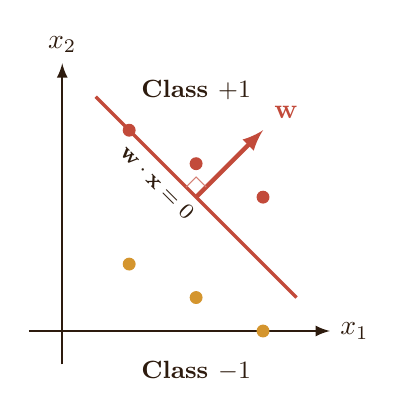
\begin{tikzpicture}[scale=0.85, >=latex]

    % Eixos Cartesianos Estabilizados com a cor contrastante do texto
    \draw[->, thick, wp-text] (-0.5,0) -- (4,0) node[right, font=\normalsize\bfseries]{$x_1$};
    \draw[->, thick, wp-text] (0,-0.5) -- (0,4) node[above, font=\normalsize\bfseries]{$x_2$};

    % Fronteira de Decisão Real (w . x + w0 = 0)
    \draw[wp-primary, very thick] (0.5,3.5) -- (3.5,0.5);
    
    % Rótulo da Fronteira reposicionado com alto contraste embaixo da linha
    \node[wp-text, font=\footnotesize\bfseries, below left, rotate=-45] at (2.2,1.8) {$\mathbf{w}\cdot\mathbf{x}=0$};

    % --- ANCORAGEM DO VETOR NORMAL (w) ---
    % Definimos a origem exatamente no centro geométrico da reta (2, 2)
    \coordinate (origen_w) at (2,2);
    \draw[->, wp-primary, ultra thick] (origen_w) -- ++(1,1) node[above right, font=\normalsize\bfseries] {$\mathbf{w}$};
    
    % Símbolo de Ângulo Reto (90º) para provar a ortogonalidade matematicamente
    \draw[wp-primary!70, thin] (2,2) ++(0.15,0.15) -- ++(-0.15,0.15) -- ++(-0.15,-0.15);
    
    % Amostras de Treino: Classe +1 (Terracotta)
    \filldraw[wp-primary] (1,3) circle (2.5pt);
    \filldraw[wp-primary] (2,2.5) circle (2.5pt);
    \filldraw[wp-primary] (3,2) circle (2.5pt);
    
    % Amostras de Treino: Classe -1 (Ocre/Gold)
    \filldraw[wp-accent] (1,1) circle (2.5pt);
    \filldraw[wp-accent] (2,0.5) circle (2.5pt);
    \filldraw[wp-accent] (3,0) circle (2.5pt);
    
    % Legendas de mapeamento de classes reposicionadas e ampliadas para legibilidade máxima
    % Agora flutuam de forma centralizada acima/abaixo dos agrupamentos de pontos
    \node[wp-text, font=\small\bfseries] at (2.0,3.6) {Class $+1$};
    \node[wp-text, font=\small\bfseries] at (2.0,-0.6) {Class $-1$};

\end{tikzpicture}
\caption{Geometric representation of a linear decision boundary in $\mathbb{R}^2$ where the weight 
vector $\mathbf{w}$ acts orthogonal to the separating hyperplane.}

\label{fig:cartesian_boundary}
\end{marginfigure}


\begin{marginfigure}[-2.0cm]
\centering
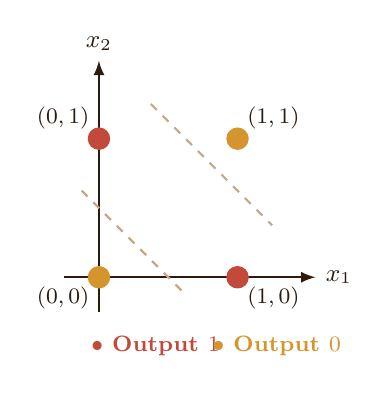
\begin{tikzpicture}[scale=1.1, >=latex]

    % Grid cartesiano simplificado com espaçamento extra para os eixos respirarem
    \draw[->, thick, wp-text] (-0.4,0) -- (2.5,0) node[right, font=\small\bfseries]{$x_1$};
    \draw[->, thick, wp-text] (0,-0.4) -- (0,2.5) node[above, font=\small\bfseries]{$x_2$};

    % --- DISTRIBUIÇÃO DOS PONTOS DE DADOS E COORDENADAS ---
    % Pontos do XOR (0,0) e (1,1) -> Output 0 (Ocre/Gold)
    \filldraw[wp-accent] (0,0) circle (3.5pt);
    \node[wp-text, font=\footnotesize\bfseries, below left] at (0,0) {$(0,0)$};
    
    \filldraw[wp-accent] (1.6,1.6) circle (3.5pt);
    \node[wp-text, font=\footnotesize\bfseries, above right] at (1.6,1.6) {$(1,1)$};
    
    % Pontos do XOR (1,0) e (0,1) -> Output 1 (Terracotta)
    \filldraw[wp-primary] (1.6,0) circle (3.5pt);
    \node[wp-text, font=\footnotesize\bfseries, below right] at (1.6,0) {$(1,0)$};
    
    \filldraw[wp-primary] (0,1.6) circle (3.5pt);
    \node[wp-text, font=\footnotesize\bfseries, above left] at (0,1.6) {$(0,1)$};

    % --- FRONTEIRAS LINEARES FRACASSADAS (Hiperplanos de tentativa) ---
    % Perfeitamente calibradas e paralelas para cortar os canais vazios das diagonais
    \draw[dashed, wp-muted, thick] (-0.2,1.0) -- (1.0,-0.2);
    \draw[dashed, wp-muted, thick] (0.6,2.0) -- (2.0,0.6);

    % --- CHAVE DE LEGENDA INFERIOR MODULAR ---
    % Posicionada abaixo do gráfico para eliminar completamente a poluição visual superior
    \node[wp-primary, font=\footnotesize\bfseries, anchor=west] at (-0.2,-0.8) {$\bullet$ Output $1$};
    \node[wp-accent, font=\footnotesize\bfseries, anchor=west] at (1.2,-0.8) {$\bullet$ Output $0$};

\end{tikzpicture}
\caption{The XOR non-linear separability dilemma. No single linear hyperplane $\{\mathbf{x} : \mathbf{w}\cdot\mathbf{x}=0\}$ can 
isolate the heterogeneous activation pairs simultaneously.}
\label{fig:xor_problem}
\end{marginfigure}

\subsection{Learning Rules}

\subsubsection{Perceptron Training Rule}
Given a training set $\mathcal{D} = \{(\mathbf{x}_d, t_d)\}_{d=1}^N$, the perceptron updates weights when a misclassification occurs:
$$
w_i \leftarrow w_i + \eta\,(t_d - o_d)\,x_{i,d},
$$
with learning rate $\eta>0$. This converges if the data are linearly separable.

\begin{figure}[h]
\noindent\raggedright\setlength{\leftskip}{0pt}\begin{adjustbox}{max width=\textwidth}
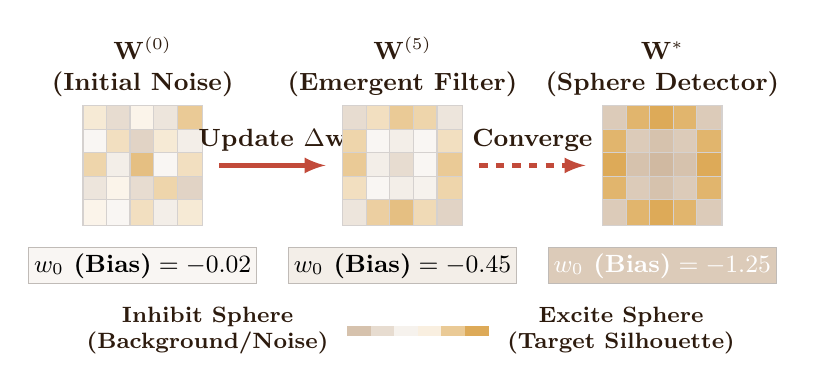
\begin{tikzpicture}[
    scale=0.75,
    >=latex,
    trim left=-1.46cm,
    % Cell styles for the 5x5 mini-grid
    p/.style={draw=wp-text!20, minimum size=0.32cm, inner sep=0pt},
    labelstyle/.style={font=\small\bfseries, text=wp-text},
    headerstyle/.style={font=\small\bfseries, text=wp-text, align=center, anchor=south, yshift=0.15cm}
  ]

  % =========================================================================
  % EPOCH 0: RANDOM INITIALIZATION
  % =========================================================================
  \begin{scope}[shift={(0,0)}]
    \node[headerstyle] at (0,0.8) {$\mathbf{W}^{(0)}$ \\ (Initial Noise)};
    \matrix [matrix of nodes, nodes={p}, column sep=-1pt, row sep=-1pt] (m0) {
      |[fill=wp-accent!20]| & |[fill=wp-muted!40]|  & |[fill=wp-accent!10]| & |[fill=wp-muted!30]|  & |[fill=wp-accent!50]| \\
      |[fill=wp-muted!10]|  & |[fill=wp-accent!30]|  & |[fill=wp-muted!50]|  & |[fill=wp-accent!20]|  & |[fill=wp-muted!20]|  \\
      |[fill=wp-accent!40]| & |[fill=wp-muted!20]|  & |[fill=wp-accent!60]| & |[fill=wp-muted!10]|  & |[fill=wp-accent!30]| \\
      |[fill=wp-muted!30]|  & |[fill=wp-accent!10]|  & |[fill=wp-muted!40]|  & |[fill=wp-accent!40]|  & |[fill=wp-muted!50]|  \\
      |[fill=wp-accent!10]| & |[fill=wp-muted!10]|  & |[fill=wp-accent!30]| & |[fill=wp-muted!20]|  & |[fill=wp-accent!20]| \\
    };
    \node[draw=wp-text!30, fill=wp-muted!10, font=\small\bfseries, minimum width=1.8cm, inner sep=2pt, below=0.15cm of m0] {$w_0 \text{ (Bias)} = -0.02$};
  \end{scope}

  % Flow Arrow 1
  \draw[->, ultra thick, wp-primary] (1.3,0) -- (3.1,0) node[midway, above, font=\small\bfseries, text=wp-text, yshift=1pt] {Update $\Delta\mathbf{w}$};

  % =========================================================================
  % EPOCH 5: INTERMEDIATE LEARNING
  % =========================================================================
  \begin{scope}[shift={(4.4,0)}]
    \node[headerstyle] at (0,0.8) {$\mathbf{W}^{(5)}$ \\ (Emergent Filter)};
    \matrix [matrix of nodes, nodes={p}, column sep=-1pt, row sep=-1pt] (m5) {
      |[fill=wp-muted!40]|  & |[fill=wp-accent!30]|  & |[fill=wp-accent!50]| & |[fill=wp-accent!40]|  & |[fill=wp-muted!30]|  \\
      |[fill=wp-accent!40]| & |[fill=wp-muted!10]|  & |[fill=wp-muted!20]|  & |[fill=wp-muted!10]|  & |[fill=wp-accent!30]| \\
      |[fill=wp-accent!50]| & |[fill=wp-muted!20]|  & |[fill=wp-muted!40]|  & |[fill=wp-muted!10]|  & |[fill=wp-accent!50]| \\
      |[fill=wp-accent!30]| & |[fill=wp-muted!10]|  & |[fill=wp-muted!20]|  & |[fill=wp-muted!15]|  & |[fill=wp-accent!40]| \\
      |[fill=wp-muted!30]|  & |[fill=wp-accent!45]|  & |[fill=wp-accent!60]| & |[fill=wp-accent!35]|  & |[fill=wp-muted!50]|  \\
    };
    \node[draw=wp-text!30, fill=wp-muted!20, font=\small\bfseries, minimum width=1.8cm, inner sep=2pt, below=0.15cm of m5] {$w_0 \text{ (Bias)} = -0.45$};
  \end{scope}

  % Flow Arrow 2
  \draw[->, ultra thick, wp-primary, dashed] (5.7,0) -- (7.5,0) node[midway, above, font=\small\bfseries, text=wp-text, yshift=1pt] {Converge};

  % =========================================================================
  % CONVERGED FINAL STATE: SPHERE TEMPLATE
  % =========================================================================
  \begin{scope}[shift={(8.8,0)}]
    \node[headerstyle] at (0,0.8) {$\mathbf{W}^*$ \\ (Sphere Detector)};
    \matrix [matrix of nodes, nodes={p}, column sep=-1pt, row sep=-1pt] (mf) {
      |[fill=wp-muted!60]|  & |[fill=wp-accent!70]|  & |[fill=wp-accent!80]| & |[fill=wp-accent!70]|  & |[fill=wp-muted!60]|  \\
      |[fill=wp-accent!70]| & |[fill=wp-muted!60]|  & |[fill=wp-muted!70]|  & |[fill=wp-muted!60]|  & |[fill=wp-accent!70]| \\
      |[fill=wp-accent!80]| & |[fill=wp-muted!70]|  & |[fill=wp-muted!80]|  & |[fill=wp-muted!70]|  & |[fill=wp-accent!80]| \\
      |[fill=wp-accent!70]| & |[fill=wp-muted!60]|  & |[fill=wp-muted!70]|  & |[fill=wp-muted!60]|  & |[fill=wp-accent!70]| \\
      |[fill=wp-muted!60]|  & |[fill=wp-accent!70]|  & |[fill=wp-accent!80]| & |[fill=wp-accent!70]|  & |[fill=wp-muted!60]|  \\
    };
    \node[draw=wp-text!30, fill=wp-muted!60, text=white, font=\small\bfseries, minimum width=1.8cm, inner sep=2pt, below=0.15cm of mf] {$w_0 \text{ (Bias)} = -1.25$};
  \end{scope}

  % =========================================================================
  % ADJUSTED LEGEND BAR
  % =========================================================================
  \begin{scope}[shift={(3.46, -2.8)}]
    \node[anchor=east, font=\footnotesize\bfseries, text=wp-text, align=center] at (-0.15, 0) {Inhibit Sphere \\(Background/Noise)};
    \fill[wp-muted!70] (0, -0.08) rectangle (0.4, 0.08);
    \fill[wp-muted!40] (0.4, -0.08) rectangle (0.8, 0.08);
    \fill[wp-muted!15] (0.8, -0.08) rectangle (1.2, 0.08);
    \fill[wp-accent!15] (1.2, -0.08) rectangle (1.6, 0.08);
    \fill[wp-accent!50] (1.6, -0.08) rectangle (2.0, 0.08);
    \fill[wp-accent!80] (2.0, -0.08) rectangle (2.4, 0.08);
    \node[anchor=west, font=\footnotesize\bfseries, text=wp-text, align=center] at (2.55, 0) {Excite Sphere \\(Target Silhouette)};
  \end{scope}

\end{tikzpicture}
\end{adjustbox}
\end{figure}
Spatial evolution of perceptron weight updates during shape classification. 
Over training iterations, the weight matrix transitions from unstructured noise ($\mathbf{W}^{(0)}$) to an 
interpretable morphology ($\mathbf{W}^*$). The converged state functions as a spatial template matcher, 
where pixels tracking the circular boundary develop strong excitatory values (gold) while the surrounding 
corners and center become strongly inhibitory (muted earth tones).s

\subsubsection{Delta Rule and Gradient Descent}
For a linear unit $o = \mathbf{w}\cdot\mathbf{x}$ (no threshold), the squared error is
$$
E(\mathbf{w}) = \frac{1}{2}\sum_{d=1}^N (t_d - o_d)^2.
$$
The gradient is $\nabla E = -\sum_d (t_d - o_d)\mathbf{x}_d$, yielding the batch gradient descent update:
$$
\mathbf{w} \leftarrow \mathbf{w} + \eta \sum_{d=1}^N (t_d - o_d)\mathbf{x}_d.
$$

\begin{remark}[Connection to MLE]
    For a linear regression model $y = \mathbf{w}^{\mathsf{T}}\mathbf{x} + \varepsilon$ with $\varepsilon \sim \mathcal{N}(0,\sigma^2)$, 
    the negative log‑likelihood is $\frac{1}{2\sigma^2}\sum (y_i - \mathbf{w}^{\mathsf{T}}\mathbf{x}_i)^2 + \text{const}$. 
    Minimising the squared error is therefore equivalent to maximum likelihood estimation under a Gaussian noise model.
\end{remark}

\begin{marginfigure}
\centering
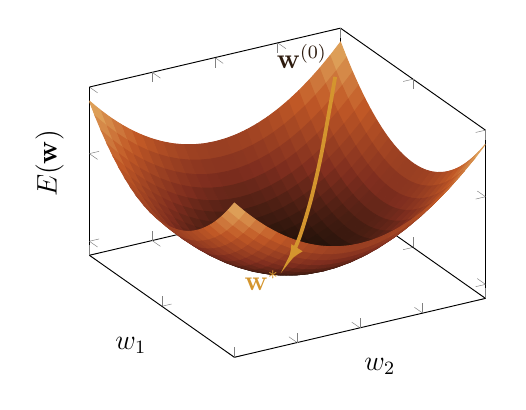
\begin{tikzpicture}[scale=0.85]
    \begin{axis}[
        view={60}{35}, 
        width=7.5cm, height=6.5cm,
        xlabel={$w_1$}, ylabel={$w_2$}, zlabel={$E(\mathbf{w})$},
        font=\large\bfseries,
        xticklabels={}, 
        yticklabels={}, 
        zticklabels={},
        colormap={warm-gradient}{
            rgb(0cm)=(0.1,0.06,0.03)
            rgb(1cm)=(0.5,0.18,0.12)
            rgb(2cm)=(0.76,0.35,0.15)
            rgb(3cm)=(0.9,0.7,0.4)
        },
    ]
        \addplot3[
            surf,
            shader=flat,
            samples=25,
            domain=-2:2,
            domain y=-2:2,
        ] {x^2 + y^2};

        \addplot3[
            ultra thick,
            wp-accent,
            -latex,
            smooth
        ] coordinates {
            (-1.8, 1.8, 6.48)
            (-1.3, 1.3, 3.38)
            (-0.9, 0.9, 1.62)
            (-0.5, 0.5, 0.50)
            (-0.2, 0.2, 0.08)
            (0.0, 0.0, 0.00)
        };
        
        \node[wp-text, font=\large\bfseries, above left] at (axis cs:-1.8, 1.8, 6.48) {$\mathbf{w}^{(0)}$};
        \node[wp-accent, font=\large\bfseries, below left] at (axis cs:0.0, 0.0, 0.0) {$\mathbf{w}^*$};
    \end{axis}
\end{tikzpicture}
\caption{3D Loss Surface}
\label{fig:loss_3d}
\end{marginfigure}


\subsubsection{Stochastic Gradient Descent (SGD)}
For large datasets, we use stochastic updates:
\[
\mathbf{w} \leftarrow \mathbf{w} - \eta \nabla \ell_i(\mathbf{w}),\qquad i \sim \text{Uniform}\{1,\dots,N\},
\]
or mini‑batch updates. SGD introduces noise that can help escape shallow local minima.

\begin{marginfigure}
\centering
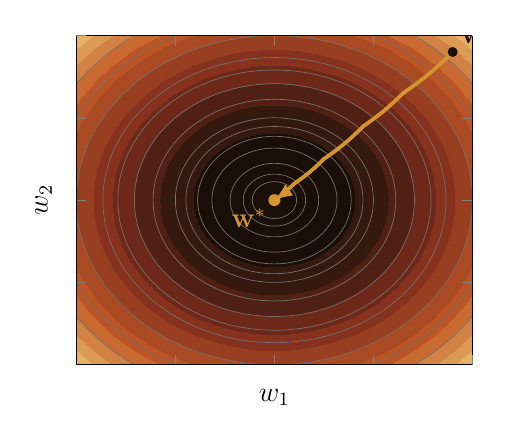
\begin{tikzpicture}[scale=0.85]
    \begin{axis}[
        view={0}{90}, 
        width=7.5cm, height=6.5cm,
        xlabel={$w_1$}, ylabel={$w_2$},
        font=\large\bfseries,
        xticklabels={}, 
        yticklabels={},
        colormap={warm-gradient}{
            rgb(0cm)=(0.1,0.06,0.03)
            rgb(1cm)=(0.5,0.18,0.12)
            rgb(2cm)=(0.76,0.35,0.15)
            rgb(3cm)=(0.9,0.7,0.4)
        },
        axis background/.style={fill=white}
    ]
        \addplot3[
            contour filled={
                number=12,
                labels=false,
            },
            draw=none,
            samples=45,
            domain=-2:2,
            domain y=-2:2
        ] {x^2 + y^2};

        % Contour lines at specific levels (simulating contour gnuplot)
        \draw[wp-dark!60, line width=0.3pt] (axis cs:0,0) circle[radius=0.224];
        \draw[wp-dark!60, line width=0.3pt] (axis cs:0,0) circle[radius=0.316];
        \draw[wp-dark!60, line width=0.3pt] (axis cs:0,0) circle[radius=0.447];
        \draw[wp-dark!60, line width=0.3pt] (axis cs:0,0) circle[radius=0.632];
        \draw[wp-dark!60, line width=0.3pt] (axis cs:0,0) circle[radius=0.775];
        \draw[wp-dark!60, line width=0.3pt] (axis cs:0,0) circle[radius=0.894];
        \draw[wp-dark!60, line width=0.3pt] (axis cs:0,0) circle[radius=1.0];
        \draw[wp-dark!60, line width=0.3pt] (axis cs:0,0) circle[radius=1.225];
        \draw[wp-dark!60, line width=0.3pt] (axis cs:0,0) circle[radius=1.414];
        \draw[wp-dark!60, line width=0.3pt] (axis cs:0,0) circle[radius=1.581];
        \draw[wp-dark!60, line width=0.3pt] (axis cs:0,0) circle[radius=1.732];
        \draw[wp-dark!60, line width=0.3pt] (axis cs:0,0) circle[radius=2.0];
        \draw[wp-dark!60, line width=0.3pt] (axis cs:0,0) circle[radius=2.236];
        \draw[wp-dark!60, line width=0.3pt] (axis cs:0,0) circle[radius=2.449];

        % Caminho de Otimização em 2D
        \draw[ultra thick, wp-accent, -latex] (axis cs:1.8, 1.8) 
            to[bend left=5] (axis cs:1.3, 1.3)
            to[bend left=5] (axis cs:0.9, 0.9)
            to[bend left=5] (axis cs:0.5, 0.5)
            to[bend left=5] (axis cs:0.2, 0.2)
            to[bend left=5] (axis cs:0.0, 0.0);

        \node[circle, fill=wp-dark, inner sep=1.5pt] at (axis cs:1.8, 1.8) {};
        \node[wp-dark, font=\large\bfseries, above right] at (axis cs:1.8, 1.8) {$\mathbf{w}^{(0)}$};
        
        \node[circle, fill=wp-accent, inner sep=1.8pt] at (axis cs:0.0, 0.0) {};
        \node[wp-accent, font=\large\bfseries, below left] at (axis cs:0.0, 0.0) {$\mathbf{w}^*$};
        
    \end{axis}
\end{tikzpicture}
\caption{2D Contour Optimization}
\label{fig:contour_2d}
\end{marginfigure}


\subsection{Activation Functions}

For multilayer networks, we need nonlinear, differentiable activation functions. Common choices are:

\begin{itemize}
    \item \textbf{Sigmoid}: $\sigma(z) = \frac{1}{1+e^{-z}}$, outputs in $(0,1)$. Smooth but saturates for large $|z|$, causing vanishing gradients.
    \item \textbf{Hyperbolic tangent (tanh)}: $\tanh(z) = \frac{e^{z}-e^{-z}}{e^{z}+e^{-z}}$, outputs in $(-1,1)$. Zero-centered, which helps optimisation, but still saturates.
    \item \textbf{Rectified Linear Unit (ReLU)}: $\text{ReLU}(z) = \max(0,z)$. Non-saturating for $z>0$, computationally efficient, but can cause “dying neurons”.
    \item \textbf{Leaky ReLU}: $\text{LeakyReLU}(z) = \max(\alpha z, z)$ with a small slope $\alpha$ (e.g., $0.01$) for $z<0$, mitigating the dying ReLU problem.
\end{itemize}

\begin{defn}[Sigmoid]
    \[
    \sigma(z) = \frac{1}{1+e^{-z}},\quad \sigma'(z) = \sigma(z)(1-\sigma(z)).
    \]
\end{defn}
\begin{defn}[Hyperbolic Tangent (Tanh)]
    \[
    \tanh(z) = \frac{e^{z}-e^{-z}}{e^{z}+e^{-z}},\quad \tanh'(z) = 1 - \tanh^2(z).
    \]
\end{defn}
\begin{defn}[Rectified Linear Unit (ReLU)]
    \[
    \text{ReLU}(z) = \max(0,z),\quad \text{ReLU}'(z) = \begin{cases} 1 & \text{if } z>0,\\ 0 & \text{otherwise.} \end{cases}
    \]
\end{defn}

ReLU is widely used because it avoids vanishing gradients for positive inputs, though it can cause “dying ReLU” problems.

\begin{figure}[h]
\centering
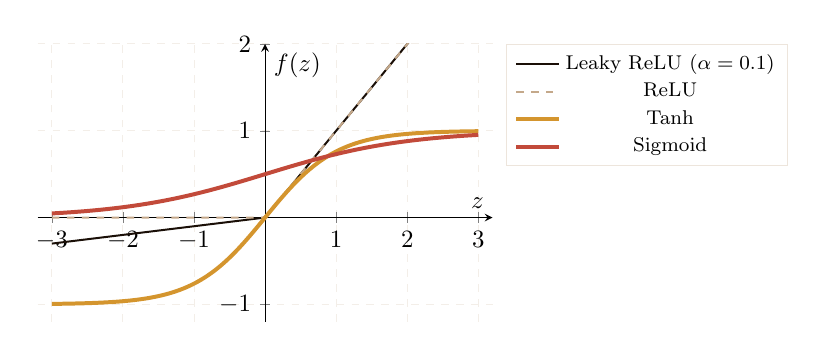
\begin{tikzpicture}[scale=0.9, thick]
    \begin{axis}[
        width=8cm, height=5.5cm,
        xlabel={$z$},
        ylabel={$f(z)$},
        domain=-3:3,
        samples=150, % Aumentado para suavizar as curvas
        axis lines=middle,
        ymin=-1.2, ymax=2.0, % Fixa os limites verticais para melhor proporção
        xmin=-3.2, xmax=3.2,
        grid=major,
        grid style={dashed, wp-muted!20}, % Grade sutil usando sua cor muted
        legend pos=outer north east,
        legend style={font=\footnotesize, draw=wp-muted!30}
    ]
        % 1. Leaky ReLU (Desenhada primeiro para ficar ao fundo no quadrante positivo)
        \addplot[wp-dark, thick] {max(0.1*x,x)};
        
        % 2. ReLU (Como ela zera em x < 0, o tracejado vai aparecer perfeitamente sobre a Leaky ReLU)
        \addplot[wp-muted, thick, dashed] {max(0,x)};
        
        % 3. Tanh (Curvas suaves por cima para manter o destaque)
        \addplot[wp-accent, ultra thick] {tanh(x)};
        
        % 4. Sigmoid
        \addplot[wp-primary, ultra thick] {1 / (1 + exp(-x))};
        
        \legend{Leaky ReLU ($\alpha=0.1$), ReLU, Tanh, Sigmoid}

    \end{axis}
\end{tikzpicture}
\caption{Common activation networks used in neural networks. Sigmoid and tanh saturate, while ReLU and Leaky ReLU are piecewise linear.}
\label{fig:activations}
\end{figure}

\subsection{Multilayer Perceptron and Backpropagation}

A multilayer perceptron (MLP) consists of an input layer, one or more hidden layers, and an output layer. Let $\mathbf{o}^{(\ell)}$ 
denote the activations of layer $\ell$, with $\mathbf{o}^{(0)} = \mathbf{x}$. For each layer $\ell=1,\dots,L$,
\[
\mathbf{a}^{(\ell)} = \mathbf{W}^{(\ell)}\mathbf{o}^{(\ell-1)} + \mathbf{b}^{(\ell)},\qquad 
\mathbf{o}^{(\ell)} = f^{(\ell)}(\mathbf{a}^{(\ell)}),
\]
where $f^{(\ell)}$ is an activation function (applied elementwise), $\mathbf{W}^{(\ell)}$ is the weight matrix, and $\mathbf{b}^{(\ell)}$ the bias vector.

\subsubsection{Backpropagation Derivation}

We minimise a loss function $\mathcal{L}(\mathbf{y}, \hat{\mathbf{y}})$ where $\hat{\mathbf{y}} = \mathbf{o}^{(L)}$. For a single example with target $\mathbf{t}$, define the error at the output layer as the derivative of $\mathcal{L}$ with respect to the pre‑activation $\mathbf{a}^{(L)}$:
\[
\boldsymbol{\delta}^{(L)} = \frac{\partial \mathcal{L}}{\partial \mathbf{a}^{(L)}} = \nabla_{\hat{\mathbf{y}}}\mathcal{L} \odot f^{(L)'}(\mathbf{a}^{(L)}),
\]
where $\odot$ is elementwise multiplication. For the squared loss $\mathcal{L} = \frac{1}{2}\|\mathbf{t}-\hat{\mathbf{y}}\|^2$, we have $\nabla_{\hat{\mathbf{y}}}\mathcal{L} = \hat{\mathbf{y}} - \mathbf{t}$.

For earlier layers, the chain rule gives
\[
\boldsymbol{\delta}^{(\ell)} = \left( (\mathbf{W}^{(\ell+1)})^{\mathsf{T}} \boldsymbol{\delta}^{(\ell+1)} \right) \odot f^{(\ell)'}(\mathbf{a}^{(\ell)}),\quad \ell = L-1,\dots,1.
\]
The gradients with respect to weights and biases are
\[
\frac{\partial \mathcal{L}}{\partial \mathbf{W}^{(\ell)}} = \boldsymbol{\delta}^{(\ell)} (\mathbf{o}^{(\ell-1)})^{\mathsf{T}},\qquad
\frac{\partial \mathcal{L}}{\partial \mathbf{b}^{(\ell)}} = \boldsymbol{\delta}^{(\ell)}.
\]

We then update parameters using SGD (or its variants).

\begin{algorithm}[h]
    \caption{Backpropagation (online / mini‑batch)}
    \begin{algorithmic}[1]
        \STATE Initialize all weights $\mathbf{W}^{(\ell)}$ and biases $\mathbf{b}^{(\ell)}$ (e.g., Xavier/He).
        \FOR{each mini‑batch $\mathcal{B}$}
            \FOR{$\ell = 1$ to $L$} \STATE \textbf{Forward:} $\mathbf{a}^{(\ell)} = \mathbf{W}^{(\ell)}\mathbf{o}^{(\ell-1)} + \mathbf{b}^{(\ell)}$, $\mathbf{o}^{(\ell)} = f^{(\ell)}(\mathbf{a}^{(\ell)})$ \ENDFOR
            \STATE Compute loss $\mathcal{L}(\mathbf{o}^{(L)}, \mathbf{t})$ for the batch.
            \STATE $\boldsymbol{\delta}^{(L)} = \nabla_{\mathbf{o}^{(L)}}\mathcal{L} \odot f^{(L)'}(\mathbf{a}^{(L)})$
            \FOR{$\ell = L-1$ down to $1$}
                \STATE $\boldsymbol{\delta}^{(\ell)} = \left( (\mathbf{W}^{(\ell+1)})^{\mathsf{T}} \boldsymbol{\delta}^{(\ell+1)} \right) \odot f^{(\ell)'}(\mathbf{a}^{(\ell)})$
            \ENDFOR
            \FOR{$\ell = 1$ to $L$}
                \STATE $\mathbf{W}^{(\ell)} \leftarrow \mathbf{W}^{(\ell)} - \eta \frac{1}{|\mathcal{B}|} \sum \boldsymbol{\delta}^{(\ell)} (\mathbf{o}^{(\ell-1)})^{\mathsf{T}}$
                \STATE $\mathbf{b}^{(\ell)} \leftarrow \mathbf{b}^{(\ell)} - \eta \frac{1}{|\mathcal{B}|} \sum \boldsymbol{\delta}^{(\ell)}$
            \ENDFOR
        \ENDFOR
    \end{algorithmic}
\end{algorithm}

\subsection{Advanced Optimization Methods}

Plain SGD often converges slowly. Modern deep learning uses adaptive methods:

\begin{itemize}
    \item \textbf{Momentum}: accumulates a velocity term $v_t = \gamma v_{t-1} + \eta \nabla \mathcal{L}$, damping oscillations.
    \item \textbf{Adam} (Adaptive Moment Estimation): maintains per‑parameter learning rates using first and second moments of gradients.
    \item \textbf{Learning rate schedules}: step decay, cosine annealing, warmup.
\end{itemize}

\begin{remark}
    Adam is often the default choice for training deep networks, though SGD with momentum can generalise better in some tasks.
\end{remark}

\subsection{Regularization for Neural Networks}

Deep models have many parameters and easily overfit. Common regularization techniques include:

\subsubsection{L2 Regularization (Weight Decay)}
Adds a penalty $\frac{\lambda}{2}\|\mathbf{w}\|_2^2$ to the loss. From a Bayesian perspective, this corresponds to a Gaussian prior on weights (MAP estimation).

\subsubsection{Dropout}
Randomly sets a fraction $p$ of neurons to zero during each training forward pass. This prevents co‑adaptation and can be interpreted as training an ensemble of subnetworks.

\subsubsection{Batch Normalization (BatchNorm)}
Normalizes layer inputs to have zero mean and unit variance across the mini‑batch. It accelerates training and acts as a regularizer. For a mini‑batch $\mathcal{B}$, compute
\[
\mu_{\mathcal{B}} = \frac{1}{|\mathcal{B}|}\sum_{i\in\mathcal{B}} a_i,\quad \sigma_{\mathcal{B}}^2 = \frac{1}{|\mathcal{B}|}\sum_{i\in\mathcal{B}} (a_i-\mu_{\mathcal{B}})^2,\quad \hat{a}_i = \frac{a_i-\mu_{\mathcal{B}}}{\sqrt{\sigma_{\mathcal{B}}^2+\epsilon}},\quad \tilde{a}_i = \gamma \hat{a}_i + \beta.
\]

\subsubsection{Early Stopping}
Monitor validation error and stop training when it stops improving; this implicitly regularizes by limiting the effective capacity.

\subsection{Bias–Variance Tradeoff in Neural Networks}

Recall from statistical learning the decomposition for squared loss:
\[
\mathbb{E}_{\mathcal{D}}[R(h_{\mathcal{D}})] = \underbrace{(\mathbb{E}_{\mathcal{D}}[h_{\mathcal{D}}] - h^*)^2}_{\text{bias}^2} + \underbrace{\mathbb{V}_{\mathcal{D}}[h_{\mathcal{D}}]}_{\text{variance}} + \text{noise}.
\]

\begin{marginfigure}
\centering
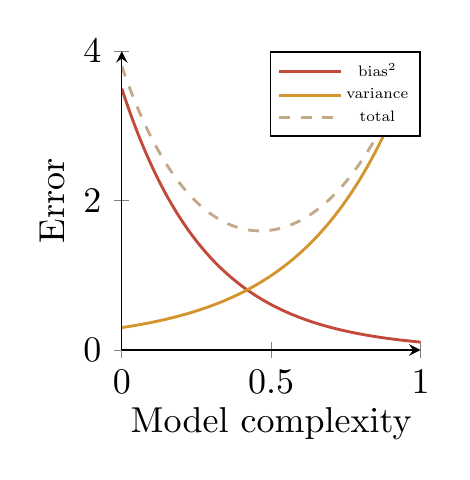
\begin{tikzpicture}[scale=1.3]
    \begin{axis}[
        width=4.5cm, height=4.5cm, 
        xlabel=Model complexity, 
        ylabel=Error, 
        domain=0:1, 
        samples=100,
        xmin=0, xmax=1,
        ymin=0, ymax=4,
        xtick={0, 0.5, 1},
        ytick={0, 2, 4},
        axis x line=bottom, 
        axis y line=left, 
        enlargelimits=false, % Desativado para os eixos começarem cravados no zero
        xlabel style={at={(axis description cs:0.5,-0.15)}, anchor=north},
        ylabel style={at={(axis description cs:-0.15,0.5)}, anchor=south}, % Corrigido o espelhamento do texto
        legend style={
            font=\scriptsize, % Define o tamanho da fonte da legenda
            nodes={scale=0.6, transform shape}, % Reduz o tamanho do texto e dos símbolos
            inner sep=2pt, % Diminui o espaçamento interno da caixa da legenda
            at={(1,1)}, 
            anchor=north east
        }]
        % 1. BIAS^2: Decai exponencialmente conforme o modelo ganha capacidade
        \addplot[wp-primary, thick] {3.5 * exp(-3.5*x)}; 
        
        % 2. VARIANCE: Cresce exponencialmente conforme o modelo ganha capacidade
        \addplot[wp-accent, thick] {0.1 + 0.2 * exp(3*x)}; 
        
        % 3. TOTAL ERROR: A soma de ambos cria a parábola/curva em U perfeita
        \addplot[wp-muted, thick, dashed] {3.5 * exp(-3.5*x) + 0.1 + 0.2 * exp(3*x)}; 
        
        \legend{bias$^2$, variance, total};
    \end{axis}
\end{tikzpicture}
\caption{Bias-variance tradeoff: total error has a minimum at optimal capacity.}
\label{fig:bias_variance_tradeoff}
\end{marginfigure}

In neural networks, model capacity increases with the number of layers and neurons. Low capacity → high bias (underfitting). High capacity → low bias but high variance (overfitting). Regularization and early stopping control the effective capacity, trading bias against variance.

\subsection{Universal Approximation Theorem}

\begin{thm}[Cybenko, 1989]
    Let $\sigma: \mathbb{R}\to\mathbb{R}$ be a continuous, bounded, non‑constant activation function (e.g., sigmoid). Then for any continuous function $f: [0,1]^d \to \mathbb{R}$ and any $\varepsilon>0$, there exist $N\in\mathbb{N}$, vectors $\mathbf{w}_j\in\mathbb{R}^d$, scalars $v_j, b_j\in\mathbb{R}$ such that
    \[
    \sup_{\mathbf{x}\in[0,1]^d} \left| \sum_{j=1}^N v_j\,\sigma(\mathbf{w}_j\cdot\mathbf{x} + b_j) - f(\mathbf{x}) \right| < \varepsilon.
    \]
\end{thm}

The theorem guarantees that a single hidden layer (with enough neurons) can approximate any continuous function arbitrarily well. However, the required $N$ may be astronomically large; depth allows more efficient representations.

\begin{figure}[h]
\centering
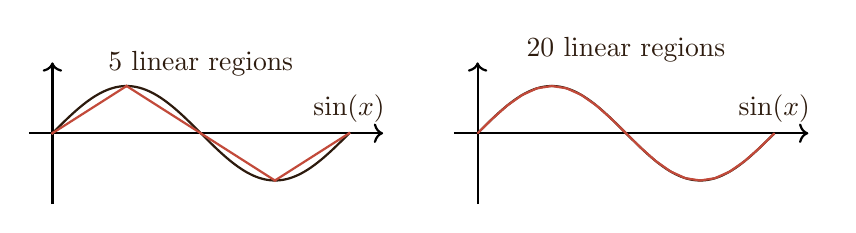
\begin{tikzpicture}[scale=.6, thick]
    % First plot: 5 linear regions
    \begin{scope}[shift={(0, 0)}]
        \draw[->] (-0.5, 0) -- (7, 0) node[right] {};
        \draw[->] (0, -1.5) -- (0, 1.5) node[above] {};
        \draw[wp-text, thick, domain=0:6.28, samples=100, smooth] plot (\x, {sin(\x r)});
        \draw[wp-primary, thick] (0, 0) -- (1.57, 1);
        \draw[wp-primary, thick] (1.57, 1) -- (3.14, 0);
        \draw[wp-primary, thick] (3.14, 0) -- (4.71, -1);
        \draw[wp-primary, thick] (4.71, -1) -- (6.28, 0);
        \node[above] at (6.28, 0) {\textcolor{wp-text}{$\sin(x)$}};
        \node[above] at (3.14, 1) {\textcolor{wp-text}{5 linear regions}};
        \foreach \x/\y in {0/0, 1.57/1, 3.14/0, 4.71/-1, 6.28/0} \fill[wp-primary] (\x, \y) circle (1pt);
    \end{scope}
    % Second plot: 20 linear regions
    \begin{scope}[shift={(9, 0)}]
        \draw[->] (-0.5, 0) -- (7, 0) node[right] {};
        \draw[->] (0, -1.5) -- (0, 1.5) node[above] {};
        \draw[wp-text, thick, domain=0:6.28, samples=100, smooth] plot (\x, {sin(\x r)});
        \foreach \i in {0,...,19} {
            \pgfmathsetmacro{\xstart}{\i * 6.28 / 20}
            \pgfmathsetmacro{\xend}{(\i + 1) * 6.28 / 20}
            \pgfmathsetmacro{\ystart}{sin(\xstart r)}
            \pgfmathsetmacro{\yend}{sin(\xend r)}
            \draw[wp-primary, thick] (\xstart, \ystart) -- (\xend, \yend);
        }
        \node[above] at (6.28, 0) {\textcolor{wp-text}{$\sin(x)$}};
        \node[above] at (3.14, 1.3) {\textcolor{wp-text}{20 linear regions}};
        \foreach \i in {0,...,20} {
            \pgfmathsetmacro{\x}{\i * 6.28 / 20}
            \pgfmathsetmacro{\y}{sin(\x r)}
            \fill[wp-primary] (\x, \y) circle (0.5pt);
        }
    \end{scope}
\end{tikzpicture}
\caption{Approximating $\sin(x)$ with piecewise linear functions: more hidden units (linear regions) give better approximation, illustrating the universal approximation theorem.}
\label{fig:UAT_fixed}
\end{figure}

\subsection{Weight Initialization}

Proper initialization is critical for deep networks. Common schemes:

\begin{itemize}
    \item \textbf{Xavier (Glorot)}: $\text{Var}[w] = \frac{2}{n_{\text{in}} + n_{\text{out}}}$ for tanh/sigmoid.
    \item \textbf{He (Kaiming)}: $\text{Var}[w] = \frac{2}{n_{\text{in}}}$ for ReLU.
\end{itemize}

These keep signals in a reasonable range and prevent vanishing/exploding gradients.

\end{document}